\documentclass{beamer}

\usepackage{amsfonts}
\usepackage{amsmath}
\usepackage{longtable}
\usepackage{csquotes}
\usepackage{standalone}

\usepackage{graphicx}
\graphicspath{{../pictures/}}

\usepackage{tikz}
\usetikzlibrary{shapes, calc, arrows, decorations.markings,
  decorations.pathmorphing, decorations, patterns, chains, snakes,
  backgrounds, positioning, fit, petri}
\newcommand{\inputpicture}[1]{\input{../drawings/#1}}

\usepackage{listings}
\lstset{language=C, basicstyle=\ttfamily, breaklines=true, keepspaces=true,
  keywordstyle=\color{blue}}

\usepackage{bytefield}

\usefonttheme{professionalfonts}
\usefonttheme{serif}
\usepackage{fontspec}
\setromanfont{CMU Serif}
\setsansfont{CMU Sans Serif}
\setmonofont{CMU Typewriter Text}

\usepackage{hyperref}
\hypersetup{colorlinks=true, linkcolor=black, filecolor=black, citecolor=black,
  urlcolor=blue , pdfauthor=Evgenii Iuliugin <yulyugin@gmail.com>,
  pdftitle=Fundamentals of Full-Platform Simulation}

\usepackage{underscore}
\usepackage{amsthm}

\subtitle{Fundamentals of Full-Platform Simulation}
\subject{Lecture}
\date{\today}

\author[Evgenii Iuliugin]{
  Evgenii Iuliugin \small{\href{mailto:yulyugin@gmail.com}{yulyugin@gmail.com}}}
\typeout{Copyright 2021 Evgenii Iuliugin}

\usetheme{Berlin}
\setbeamertemplate{navigation symbols}{}

\newcommand{\finalslide}{
    {\huge{Thank you!}\par}

    \vfill
    Slides and material are available at
    \url{https://github.com/yulyugin/sim-lectures}
    \vfill

    \tiny{\textit{Note}: All trademarks are the property of their respective
        owners.
        The presented point of view reflects the personal opinion of the author.

        %All the materials are licensed under the Creative Commons
        %Attribution-NonCommercial-ShareAlike 4.0 Worldwide. To view a copy of
        %this license, visit
        %\url{http://creativecommons.org/licenses/by-nc-sa/4.0/}.
    }
}


\title{Parallel Simulation for Multi-Processor Guest Systems}

\begin{document}

\startslides

\begin{frame}{On the Previous Lecture:}
  Programming languages for model development:
  \begin{itemize}
    \item Requirements and abstractions.
    \item Libraries: SystemC.
    \item Domain specific languages: DML, SimGen, LISA.
    \item Languages for hardware development: VHDL, Verilog.
  \end{itemize}
\end{frame}

\begin{frame}{Questions}
  \begin{itemize}
    \item What is SystemC? \pause
    \item How models written using DML are compiled? \pause
    \item What language should be used for model development?
  \end{itemize}
\end{frame}

\begin{frame}{Earlier in the Course}
  \begin{itemize}
   \item Simulation of multi-processor systems\dots\pause
   \item \dots using just one host processor core.
   \vfill
   \item $N$ target cores are simulated sequentially on $K$ host cores.
   \item Slowdown may be $> \frac{1}{N}$.
   \item At the same time $K-1$ host cores are unused.
  \end{itemize}
\end{frame}

\begin{frame}{Simulated System}
  \centering
  \inputpicture{parsim-overview}
\end{frame}

\section{Processors Simulation}

\subsection{Atomic Instructions}

\begin{frame}{Atomic Instructions}
  \centering
  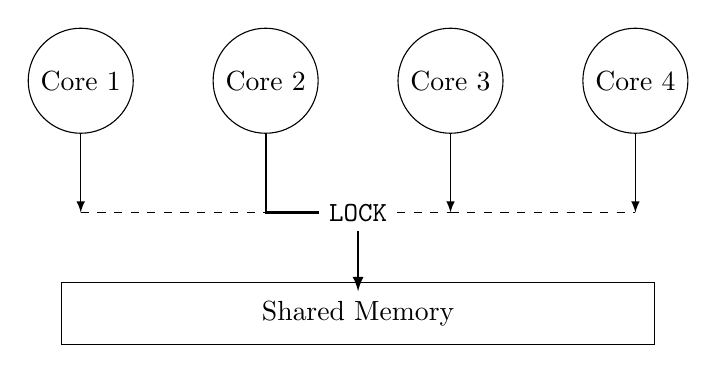
\begin{tikzpicture}[>=latex]
    \node[draw, circle] (core1) {Core 1};
    \node[draw, circle, right = of core1] (core2) {Core 2};
    \node[draw, circle, right = of core2] (core3) {Core 3};
    \node[draw, circle, right = of core3] (core4) {Core 4};

    \path (core2.south) -- (core3.south) node[midway, yshift = -1cm] (lock) {\texttt{LOCK}};
    \draw[thick] (core2) |- (lock);

    \node[below = 1cm of lock.center] (shmem) {Shared Memory};
    \node[inner ysep=0pt, below = 2cm of core1.south] (c1) {};
    \node[inner ysep=0pt, below = 2cm of core4.south] (c2) {};
    \node[draw, fit = (c1) (shmem) (c2)] {};

    \draw[thick,->] (lock) -- (shmem);

    \path (core1.south) |- (lock) coordinate[midway] (block1);
    \path (core3.south) |- (lock) coordinate[midway] (block3);
    \path (core4.south) |- (lock) coordinate[midway] (block4);

    \draw[->] (core1.south) -- (block1);
    \draw[->] (core3.south) -- (block3);
    \draw[->] (core4.south) -- (block4);

    \draw[dashed] (block1) -- (lock);
    \draw[dashed] (lock)   -- (block3);
    \draw[dashed] (block3) -- (block4);
  \end{tikzpicture}

  \begin{itemize}
    \item {Read--Modify--Write} memory.
    \item Atomic instructions --- <<all or nothing>>.
    \item Atomic instructions are <<expensive>>.\pause
    \item Question: Do single core systems need atomic operations?
  \end{itemize}
\end{frame}

\begin{frame}{Simulation of atomic instructions}
  \begin{enumerate}
    \item Using host atomic instructions.
    \begin{itemize}
      \item Different ISAs for atomic instructions (Intel IA-32 --- 10+ atomic
        instructions, ARM --- two).
      \item Useful when target and host architectures match. \pause
    \end{itemize}
    \item Using critical sections.
    \begin{itemize}
      \item Atomic instruction acquires a lock before memory access \pause
        \dots{} does not work. See~\cite{wang-coremu}.
      \item Every memory access acquires a lock --- works but slow. \pause
      \item Coherency protocols for memory regions. Like MESI for caches. \pause
    \end{itemize}
    \item Using transactions.
    \begin{itemize}
      \item Detect races instead of avoiding them.
      \item Repeat atomic operation in case of failure.
      \item Implemented using host atomic compare-and-swap.
    \end{itemize}
  \end{enumerate}
\end{frame}

\subsection{Memory Consistency Model}

\begin{frame}{Memory Consistency Model}
  \begin{itemize}
    \item There are several buffers (caches, queues) between CPU and RAM.
    \item CPUs in a shared memory system may <<see>> different values of the
      same memory location.
    \item Memory consistency model --- set of rules defining order and
      visibility of memory updates.
    \pause
    \vfill
    \item Memory barriers --- instructions to establish partial ordering for
      memory operations.
    \item Examples Intel\reg~IA-32: \texttt{sfence}, \texttt{lfence},
      \texttt{mfence}.
    \item NOTE: atomic instructions are not necessarily memory barriers!
  \end{itemize}
\end{frame}

\begin{frame}{Memory Ordering for Different Architectures}
  \centering
  % TODO: Convert the table to LaTeX
  \includegraphics[height=0.8\textheight]{barrier-arch.png}

  \tiny{Summary of memory ordering~\cite{mckenney-memory-barriers}}
\end{frame}

\section{Parallel Discrete Event Simulation}

\begin{frame}{DES}
  Multiple asynchronous devices --- DES using single thread.
  \vfill
  \centering
  \inputpicture{des}
\end{frame}

\begin{frame}{Naive PDES}
  \begin{itemize}
    \item Two target processors. Each processor has its own queue.
    \item Processors post events in other's queue for communication. \pause
    \item Causality is violated.
  \end{itemize}
  \centering
  \inputpicture{pdes-two-queues}
\end{frame}

\begin{frame}{PDES with Time Stamps}
  \begin{itemize}
    \item On send: add time stamp.
    \item On receive: check the time stamp, adjust or report an error.
  \end{itemize}
  \centering
  \inputpicture{pdes-time-stamps}
\end{frame}

\begin{frame}{Conservative and Optimistic Approaches}
  How to deal with causality violations?
  \begin{itemize}
    \item Conservative --- avoid causality violations.
    \item Optimistic --- detect and fix causality violations.
  \end{itemize}
\end{frame}

\subsection{Conservative Approach}

\begin{frame}{Conservative Approach}
  \begin{itemize}
    \item Block sender until receiver handles the connected event.
    \item Do not allow <<fast>> threads to get through communication stages.
  \end{itemize}
  \centering
  \inputpicture{pdes-send-and-block}
\end{frame}

\begin{frame}{Deadlock}
  \centering
  \inputpicture{pdes-deadlock}
\end{frame}

\begin{frame}{Recovery from Deadlocks}
  If deadlock is detected it is safe to free one of the threads:
  \begin{itemize}
    \item The best choice --- thread with the smallest simulated time.
    \item Possible situation: one thread runs most of the time, others wait
      $\Rightarrow$ no benefits from parallelism.
  \end{itemize}
\end{frame}

\begin{frame}{Is It Possible to Avoid Blocking?}
  \begin{itemize}
    \item Blocking is needed because the threads do not know each other's
      progress.
    \item How can thread A get local time of thread B? \pause
    \item Though a time stamp stored in a event from thread B.
    \item Solution: send \textit{null} message.
  \end{itemize}
\end{frame}

\begin{frame}{Synchronization Domains}
  \centering
  \inputpicture{synchronization-domains}
\end{frame}

\subsection{Optimistic Approach}

\begin{frame}{Optimistic Approach}
  \begin{enumerate}
    \item Run with no blocking,
    \item Periodically save system state,
    \item Revert to the last checkpoint if causality error is detected.
    \item Execute the problematic section using conservative approach.
  \end{enumerate}
\end{frame}

\begin{frame}{Checkpoints}
  \centering
  \inputpicture{checkpoints}
\end{frame}

\section*{Conclusion}

\begin{frame}{Parallel Simulation Problems}
  \begin{itemize}
    \item Non-deterministic execution,
    \item Parallel execution does not guarantee speedup. \pause
    \item Parallel execution can be even slower than sequential!
  \end{itemize}
\end{frame}

\begin{frame}{Is It Even Worse Trying to Parallelize?}
  \begin{itemize}
    \item Do the simulated workloads take incredibly long amount of time to
      complete?
    \item Do the simulated workloads run sequential or parallel code?
    \item Do the simulated threads interact a lot? \pause
    \item Would the amount of time it takes to build parallel simulator be
      worth the speedup?
  \end{itemize}
\end{frame}

\begin{frame}{Conclusion}
  \begin{itemize}
    \item Multi-processor simulation on multi-processor system.
    \item Parallel discrete event simulation. \pause
    \item Think well before even trying to do parallel simulation!
  \end{itemize}
\end{frame}

\begin{frame}{Parallel Simulators}
  \begin{itemize}
    \item Simics,
    \item Graphite,
    \item SimOS,
    \item Coremu,
    \item Pqemu,
    \item BigSim,
    \item DynamoRIO.
  \end{itemize}
\end{frame}

\begin{frame}[allowframebreaks]{Bibliography}
  \nocite{gharachorloo-memory-consistency}
  \nocite{ding-pqemu}
  \nocite{fujimoto-pdes}
  \nocite{liu-pdes}
  \nocite{misra-ddes}
  \printbibliography
\end{frame}

\finalslide

\end{document}
